\chapter{Cross Section Measurement}\label{chapt:xsec}

The cross section measurement procedure is explained in this section.
After applying selection criteria, performing the kinematic reconstruction and subtracting background
one can count the events to determine the rate of the $t\bar{t}$ production process.

The cross sections were measured double differentially in bins of the kinematic variables of the top-quark and the $t\bar{t}$ system.
The first section shortly describes the way how the background yields were subtracted.
The two dimensional unfolding applied to correct for the detector resolution effects and fluctuations is described
in the second section.
The double differential cross sections definitions are elucidated in the last section of the chapter.
% \section{Selection of Binning}\label{sec:binning}

\section{Background Subtraction}
The first step of the cross sections measurement is the counting of the events which fulfill certain criteria (e.g. given in 
chapter \ref{chapt:event_sel} and chapter \ref{chapt:kinReco}) and subtracting background: 

\begin{equation}\label{eq:bgsub}
 N^{signal\;measured}_{reco} = N^{selected}_{reco} - N^{BG}
\end{equation}

Here $N^{BG}$ corresponds to the estimated number of background events, except for the $t\bar{t} \rightarrow other$ events. The background sources 
were introduced in sec. \ref{sec:bg_intro}.

After subtracting all the non-$t\bar{t}$ backgrounds, the number of signal events is multiplied by a factor in each each cross section bin
individually to correct for the contribution from other $t\bar{t}$ decay channels:

\begin{equation}\label{eq:bgsub}
 N^{signal}_{reco} = N^{signal\;measured}_{reco} \cdot \frac{N^{t\bar{t} \rightarrow e\mu}_{reco}}{N^{t\bar{t} \rightarrow e\mu}_{reco} + N^{t\bar{t} \rightarrow other}_{reco}}.
\end{equation}

The factor $\frac{N^{t\bar{t} \rightarrow e\mu}_{reco}}{N^{t\bar{t} \rightarrow e\mu}_{reco} + N^{t\bar{t} \rightarrow other}_{reco}}$ was derived
from the simulated data.

%%%%%%%%%%%%%%%%%%%%%%%%%%%%%%%%%%%%%%%%%%%%
%%%%%%%%%%%%%%%%%%%%%%%%%%%%%%%%%%%%%%%%%%%%
%%%%%%%%%%%%%%%%%%%%%%%%%%%%%%%%%%%%%%%%%%%%
\section{Unfolding of the Experimental Results}\label{sec:unfold}

The signal yields after the background  subtraction \ref{eq:bgsub} are grouped to the bins in different variables. However, the kinematic properties
of the events are measured with finite precision due to inevitable detector effects and imperfect reconstruction algorithms.
Thus, some fraction of events may be reconstructed in the wrong bins. To present the results independent of the detector effects,
one needs to correct them back.

The whole problem can be described as

\begin{equation}\label{eq:UnfoldProb}
 \tilde{y}_i = \sum_{j = 1}^{m} A_{ij}\tilde{x}_{j} + b_{i}, \;\;\; 1 \leq i \leq n.
\end{equation}

Here the $\tilde{x}_j$ in $m$ bins denotes the true distribution, independent of the detector effects, which is the aim of the measurement;
$\tilde{y}_i$ in $n$ bins is the distribution which one gets out of the detector and $A_{ij}$ is a matrix of probabilities describing 
the migrations from true level bin $j$ to detector level bin $i$ to different bins on the detector level; $b_{i}$ is the background in the bin $i$. 
However, the observed event counts $y_{i}$ may be different from $\tilde{y}_{i}$ due to the statistical fluctuations.
A schematic view of the problem is given in the Figure \ref{fig:scUnf}.

\begin{figure}[t]
  \centering
  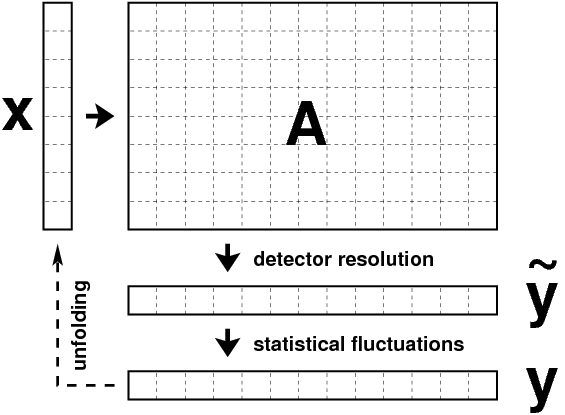
\includegraphics[width=0.4\textwidth]{06_DiffXsec/plots/d12-129f1.png}
  \caption{Schematic view of the problem of migration effects due to the finite precision of the detector and statistical 
  fluctuations. Plot taken from \cite{Schmitt:2012kp}.}
  \label{fig:scUnf}
\end{figure}

The process of estimating the true distribution $\tilde{x}_{j}$ from the observed distribution $y_{i}$ which was influenced
by detector effects and statistical fluctuations is called \textit{unfolding}. The estimated unfolded distribution is called
$x_{j}$ in the following. To suppress statistical fluctuations of imprecisely determined high frequency components of the 
solution $x$ a smoothing \textit{regularisation} procedure is applied. The TUnfold \cite{Schmitt:2012kp} algorithm was used 
for the unfolding in this analysis.

\subsection{TUnfold Minimization}\label{ssec:TUmini}

The TUnfold algorithm\cite{Schmitt:2012kp} is using a method based on least square minimization plus Tikhonov regularization 
\cite{Tikhonov:1963}. One of the ingredients for a good performance of the method is that the number of degrees of freedom 
for the minimization ($n - m$) has to be positive, or $n > m$. This means that the unfolded distribution $x_j$ will have 
coarser binning than the measured one, $y_{i}$.

The unfolding algorithm of the TUnfold determines the stationary point or minimum of the following Lagrangian:

\begin{align}
 \mathcal{L}(x, \lambda) & = \mathcal{L}_{1} + \mathcal{L}_{2} + \mathcal{L}_{3}, \;\;\;\;\;\;\;\;\;\; \textrm{where}\\
 \mathcal{L}_{1} & = (\mathbf{y} - \mathbf{A}\mathbf{x})^{T} \mathbf{V_{yy}}^{-1}(\mathbf{y} - \mathbf{A}\mathbf{x}),\\
 \mathcal{L}_{2} & = \tau^{2}(\mathbf{x} - f_{b}\mathbf{x_{0}})^{T} (\mathbf{L^{T}L}) (\mathbf{x} - f_{b}\mathbf{x_{0}}), \\
 \mathcal{L}_{3} & = \lambda(Y -\mathbf{e}^{T}\mathbf{x}) \;\;\;\;\;\;\;\;\;\;\;\;\;\;\;\; \textrm{with} \\
 Y & = \sum_{i} y_{i}, \\
 e_{j} & = \sum_{i} A_{ij}.
\end{align}

The bold symbols here correspond to matrices and vectors.

The term $\mathcal{L}_{1}$ is expected for a least square minimization. The vectors $\mathbf{y}$, $\mathbf{x}$ and the matrix $\mathbf{A}$ were
described in the previous section. Representing the migrations into different bins of $\mathbf{y}$, the matrix $\mathbf{A}$
is defined from the $t\bar{t}$ signal Monte Carlo simulation using the information from the generator particle level and on the reconstructed level. 
It describes how many migrations there are out and into a certain bin. An extra "zero`` row is added to the matrix $\mathbf{\tilde{A}}$ containing 
the information about the count of Monte Carlo events which were generated in some bin of $\mathbf{x}$, but were not reconstructed in any of the
$\mathbf{y}$ bins. The matrix $\mathbf{A}$, which enters the unfolding, is the normalized $\mathbf{\tilde{A}}$ defined as 
$\mathbf{A}_{ij} = \frac{\tilde{A}_{ij}}{\sum_{j=0}\tilde{A}_{ij}}$ (the normalization includes the "zero'' row). An example of such a matrix 
is shown in Fig. \ref{fig:migMat}. 

\begin{figure}[p]
  \centering
  \includegraphics[width=1.0\textwidth]{/home/dolinska/Dropbox/desy_plots/Thesis/Jenya/xSec/migration/probMatrix_top_arapidity_top_pt.pdf}
  \caption{Normalized migration matrix $\mathbf{A}$ (probability matrix) in bins of $p_{T}(t)$ and $|y(t)|$. The generator binning consists of
          five groups of three bins (1-3, 4-6, 7-9, 10-12, 13-15). It corresponds to the five $p_{T}(t)$ bins ($[0\:..\:65\:..\:130\:..\:200\:..\:300\:..\:500]$ GeV)
          having three $|y(t)|$ bins ($[0\:..\:0.6\:..\:1.2\:..\:2.5]$) in each $p_{T}(t)$ bin.
          Detector binning consists of
          fourteen groups of eight bins (1-8, 9-16, 17-24, 25-32, 33-40, 41-48, 49-56, 57-64, 65-72, 73-80, 81-88, 89-96, 97-104, 105-112). It corresponds 
          to fourteen $p_{T}(t)$ bins ($[0\:..\:20\:..\:35\:..\:50\:..\:65\:..\:80\:..\:100\:..\:130\:..\:145\:..\:170\:..\:200\:..\:240\:..\:300\:..\:350\:..\:500]$ GeV)
          having eight $|y(t)|$ bins ($[0.0\:..\:0.2\:..\:0.4\:..\:0.6\:..\:0.8\:..\:1.0\:..\:1.2\:..\:1.5\:..\:2.5]$) in each $p_{T}(t)$ bin.
          The matrix is obtained from the $\MG+\PYTHIA6$ $t\bar{t}$ signal sample.}
  \label{fig:migMat}
\end{figure}

% \begin{figure}[p]
%   \centering
%   \includegraphics[width=1.0\textwidth]{/home/dolinska/Dropbox/desy_plots/Thesis/Jenya/Plots/Nominal/emu/top_arapidity-top_pt/probabilityMatrix_top_arapidity_vs_top_pt.pdf}
%   \caption{Migration matrix for the bins of $p_{T}(t)$ and $|y(t)|$. The binning is the following:
%   X axis: the sequences of three bins (1-3, 4-6, 7-9, 10-12, 13-15) correspond to the $p_{T}(t)$ bins $[0\:\:65\:\:130\:\:200\:\:300\:\:500]$ GeV.
%           There are 3 $|y(t)|$ bins -- $[0\:\:0.6\:\:1.2\:\:2.5]$ -- in each $p_{T}(t)$ bin.
%   Y axis: the sequences of eight bins correspond to the $p_{T}(t)$ bins $[0\:\:20\:\:35\:\:50\:\:65\:\:80\:\:100\:\:130\:\:145\:\:170\:\:200\:\:240\:\:300\:\:350\:\:500]$ GeV.
%           There are 8 $|y(t)|$ bins -- $[0\:\:0.2\:\:0.4\:\:0.6\:\:0.8\:\:1.0\:\:1.2\:\:1.5\:\:2.5]$ -- in each $p_{T}(t)$ bin.
%   The matrix is obtained from the \MG + \PYTHIA 6 signal sample.}
%   \label{fig:migMat}
% \end{figure}

The term $\mathcal{L}_{2}$ is responsible for the regularization. It is reducing the effect of the statistical fluctuations present in $\mathbf{y}$ on high frequency
components of $\mathbf{x}$ during the search of the stationary point of the Lagrangian $\mathcal{L}$. The $\tau^{2}$ is the regularization strength. 
The matrix $\mathbf{L}$ represents the so-called regularization conditions. In this work the regularization of the second derivative of $\mathbf{x}$ is performed. 
This corresponds to the initialization of $\mathbf{L}$ matrix with three non-zero elements ($L_{i,i} = 1,\:L_{i,i+1} = -2$ and $L_{i,i+2} = 1$) and $m-2$ rows.
The quantity $f_{b}$ is a normalization 
factor and $\mathbf{x_{0}}$ is the bias vector. In this work the bias vector is taken from the signal simulation on the generator level
% In a very simple case $f_{b} = 0$, $\mathbf{L}$ is a unity matrix and $\mathcal{L}_{2} = \tau^{2} \parallel x \parallel^{2}$, which
% suppresses large deviations of $\mathbf{x}$ from zero. 
% In case $f_{b} = 1$, the deviations of $\mathbf{x}$ from $\mathbf{x_{0}}$ are
% suppressed. 
and $f_{b} = 1$ is used. It is very important to choose 
the optimal regularization strength, as a very weak strength would not damp the fluctuation effects from $\mathbf{y}$, whereas a very strong 
one will bias $\mathbf{x}$ towards $f_{b}\mathbf{x}_{0}$. The L-curve method \cite{Hansen00thel-curve} and the minimization
of correlation coefficients \cite{VBlobelT} are implemented in TUnfold for an optimal regularization strength choice. 

The idea of the L-curve method is to look at the graph $L_{x}^{curve}$ vs $L_{y}^{curve}$ and choose the $\tau$ from the point with
maximal curvature. The $L_{x}^{curve}$ and $L_{y}^{curve}$ are expressed as follows:

\begin{equation}
 L_{x}^{curve} = \log \mathcal{L}_{1},
\end{equation}

\begin{equation}
 L_{y}^{curve} = \log \frac{\mathcal{L}_{2}}{\tau^{2}}.
\end{equation}

The L-curve graph is in fact comparing the two terms of the Lagrangian: the minimization term $\mathcal{L}_{1}$ and the regularization term $\mathcal{L}_2$.
The maximum curvature point of this L-curve is a point of compromise between the size of the $\mathcal{L}_{1}$ and $\mathcal{L}_{2}$ contributions
to the total Lagrangian.

The method of minimizing the global correlation coefficients chooses the $\tau$ at the point where the average correlation coefficient 
$\sum_{i} \frac{\rho_{i}}{m}$ is minimal. Here $i$ is the component of $\mathbf{x}$ with size $m$. The correlation coefficient $\rho_{i}$ is given as follows:

\begin{equation}
 \rho_{i} = \sqrt{1 - \frac{1}{(\mathbf{V}_{xx}^{-1})_{ii} (\mathbf{V}_{xx})_{ii}}}.
\end{equation}

$\mathbf{V}_{xx}$ is the covariance matrix\footnote{The \textit{covariance matrix} of the vector $\mathbf{v}$ is the matrix in which each element with position 
$ij$ represents the covariance between the $i^{th}$ and $j^{th}$ element of the vector $\mathbf{v}$.} for $\mathbf{x}$ which is a key result of the unfolding. 
In the TUnfold this matrix is determined by error propagation from $\mathbf{V}_{yy}$:

\begin{equation}\label{eq:vxx}
 \mathbf{V}_{xx} = \mathbf{D}^{xy}\mathbf{V}_{yy}(\mathbf{D}^{xy})^{\mathbf{T}},
\end{equation}

where $(\mathbf{D}^{xy})_{ki} = \frac{\delta x_{k}}{\delta y_{i}}$ is the propagator matrix from $\mathbf{y}$ to $\mathbf{x}$. A detailed description
of how the propagation is done is documented in \cite{Schmitt:2012kp}. An example of a normalized covariance matrix is shown in Fig.\ref{fig:corr_matr}.
All covariance matrices determined in this analysis are shown in Appendix \ref{appendix:corr_m}.

\begin{figure}[t]
  \centering
  \includegraphics[width=0.7\textwidth]{/home/dolinska/Dropbox/desy_plots/Thesis/Jenya/xSec/covX/histCovXnorm_top_arapidity_vs_top_pt.pdf}
  \caption{Correlation matrix $\mathbf{V}_{xx}$ for the bins of $p_{T}(t)$ and $|y(t)|$. The binning is the following:
  the five sequences of three bins (1-3, 4-6, 7-9, 10-12, 13-15) correspond to the five $p_{T}(t)$ bins $[0\:..\:65\:..\:130\:..\:200\:..\:300\:..\:500]$ GeV.
          There are three $|y(t)|$ bins -- $[0\:..\:0.6\:..\:1.2\:..\:2.5]$ -- in each $p_{T}(t)$ bin.}
  \label{fig:corr_matr}
\end{figure}

In Fig. \ref{fig:reg_s_m} examples of the choices of regularization strength for the L-curve and minimizing global correlation coefficients 
methods are shown.

\begin{figure}[p]
\centering
\begin{subfigure}
  \centering
  \includegraphics[width=0.6\textwidth]{/home/dolinska/Dropbox/desy_plots/Thesis/Jenya/Plots/Nominal/emu/top_arapidity-top_pt/Lcurve_top_arapidity_vs_top_pt.pdf}
\end{subfigure}
\begin{subfigure}
  \centering
  \includegraphics[page=2,width=0.6\textwidth]{/home/dolinska/Dropbox/desy_plots/Thesis/Jenya/Plots/Nominal/emu/top_arapidity-top_pt/logTauRho_top_arapidity_vs_top_pt.pdf}
\end{subfigure}
\caption{Illustration of the choice of the optimal regularization strength with the L-curve method (top) and minimization of correlation coefficient
         (bottom). The red dots represent the points corresponding to the finally chosen values of $\tau$.}
\label{fig:reg_s_m}
\end{figure}

The term $\mathcal{L}_{3}$ is an orthogonal area constraint with a Lagrangian parameter $\lambda$. If $\lambda$ is not set to zero,
which means the area constraint is used, the $\mathbf{x}$ is forced to match the total event count $Y$ corrected for the efficiencies $\mathbf{e}$.
This is used to limit the normalization biases if the data $\mathbf{y}$ follow Poisson's statistics \cite{Cowan98}.

The stationary point of the Lagrangian $\mathcal{L}(\mathbf{x}, \lambda)$ is defined by setting the first derivatives to zero. In case no 
area normalization is performed, the Lagrangian $\mathcal{L}$ depends only on $\mathbf{x}$ and the $\mathcal{L}_{3}$ term is zero.

The multidimensional unfolding can be done in the TUnfold algorithm in a way that the multidimensional arrays are mapped to the one-dimensional
arrays and the unfolding is performed as described in this section.

\subsubsection{Regularization Strength Studies}

The regularization aims to minimize fluctuations effects. To check the performance of the regularization as implemented in TUnfold, the reconstructed signal
MC sample was unfolded. The outcome of this unfolding should be the generated signal distributions. The number of entries in the reconstructed signal
MC distributions were fluctuated randomly in each bin independently within the statistical uncertainties of the real data in the corresponding bin. 
These statistical uncertainties were assumed to be Gaussian. The fluctuations were performed 3000 times. Each of the 3000 fluctuated distributions 
was unfolded and the following quantities were checked:

\begin{itemize}

 \item \textbf{$\tau$ scan}. The regularization strength $\tau$ is determined using either an L-curve scan or the minimization of correlation coefficients, for each
 of the 3000 fluctuated distributions. The regularization strength distributions are shown in
 Fig. \ref{fig:tau_scan}. The regularization strength defined in the L-curve method has multiple peaks which shows an instability of the $\tau$ choice.
 Such a phenomenon is not observed for the global correlation coefficients minimization. Here a single value of the regularization strength
 is preferred for all the unfolded distributions. Thus, the minimization of the global correlation coefficients is used for the cross section determination.
 \begin{figure}[p]
 \centering
 \begin{subfigure}
  \centering
  \includegraphics[width=0.6\textwidth]{/home/dolinska/Dropbox/desy_plots/Thesis/Jenya/Plots/preunfold/emu/top_arapidity-top_pt/L-curve/tauDist_Nominal.png}
 \end{subfigure}
 \begin{subfigure}
  \centering
  \includegraphics[width=0.6\textwidth]{/home/dolinska/Dropbox/desy_plots/Thesis/Jenya/Plots/preunfold/emu/top_arapidity-top_pt/tau-scan-rho/tauDist_Nominal.png}
 \end{subfigure}
 \caption{Distribution of the regularization strength $\tau$ found in MC toy experiments with the L-curve method (top) and the minimization of correlation coefficients
         (bottom). The red line represents the regularization strength value found by the corresponding method when unfolding the real data.}
 \label{fig:tau_scan}
 \end{figure}
 
 \item \textbf{Relative difference between unfolded and generated values.} The mean number of entries in one bin determined from 3000 fluctuated and unfolded distributions
 is  compared to the number of entries in the corresponding generated distribution. The quantity which evaluates this comparison is
 $\frac{\mathbf{x} - \mathbf{x}_{0}}{\mathbf{x}_{0}}$, where $\mathbf{x}_{0}$ is the bias vector and $\mathbf{x}$ is the unfolded fluctuated signal. 
 The distributions of this quantifier in different $p_{T}(t)$ and $|y(t)|$ bins obtained using the L-curve method and minimizing the correlation coefficients 
 are shown in Fig. \ref{fig:DiffovErr}. For both methods the overall relative deviations from zero are not
 higher than 3\%, which means there are no big discrepancies in the unfolding outcome.
 \begin{figure}[t]
 \centering
 \includegraphics[width=0.6\textwidth]{/home/dolinska/Dropbox/desy_plots/Thesis/Jenya/Plots/preunfold/emu/top_arapidity-top_pt/relDiff_Nominal.pdf}
 \caption{Relative difference between unfolded and generated values for the 3000 fluctuated and unfolded reconstructed MC signal samples in bins of 
         top $p_{T}(t)$ and $y(t)$. The results obtained with the L-curve method are marked with red points and for the correlation coefficient 
         minimization with blue points.}
 \label{fig:DiffovErr}
\end{figure}
 
 \item \textbf{RMS over mean error distribution}. For each bin  each of the 3000 toy experiment results will differ. To quantify if the spread of 
 the values is not disagreeing with the statistical uncertainties, one can look at the 
 RMS (root mean square) of the values in a certain bin divided by the mean errors\footnote{The mean error for each bin is defined as an arithmetic mean 
 over the error of each of the 3000 unfolded measurements in this bin. Each particular error is derived using the $\mathbf{V}_{xx}$ (see eq. \ref{eq:vxx})
 and taking the square root of the respective diagonal element.} of these values. This value is expected to be equal to unity. The distributions 
 of the RMS over mean error in different $p_{T}(t)$ and $|y(t)|$ bins obtained using the L-curve method and minimizing the correlation coefficients 
 are shown in the Fig. \ref{fig:RMSovMeanErr}. The results obtained with the L-curve method overshoot unity. This means that the unfolded $\mathbf{x}$ 
 value for the L-curve method underestimates the errors. On the other hand, the results obtained with minimizing the global correlation coefficients 
 are in agreement with unity.
 \begin{figure}[t]
  \centering
  \includegraphics[width=0.6\textwidth]{/home/dolinska/Dropbox/desy_plots/Thesis/Jenya/Plots/preunfold/emu/top_arapidity-top_pt/rmsOverMeanError_Nominal.pdf}
  \caption{RMS over mean error for the 3000 fluctuated and unfolded reconstructed MC signal samples in bins of top $p_{T}(t)$ and $|y(t)|$. The results obtained 
          with the L-curve method are marked with red points and for the correlation coefficient minimization with blue points.}
  \label{fig:RMSovMeanErr}
 \end{figure}

\end{itemize}

As a consequence of these studies the minimization of the correlation coefficients method for the regularization strength determination was chosen
in this analysis.

\subsubsection{Closure Tests}\label{ssec:clT}

The unfolding procedure with all its assumptions should be able to reproduce distributions which are different in the shape compared to simulated $t\bar{t}$ 
signal data, from which the migration matrix for unfolding was extracted. To test this, \textit{pseudo-data} are unfolded.

The pseudo-data are created by reweighting the $t\bar{t}$ signal $\MG+\PYTHIA$ distributions in bins of $p_{T}(t)$ and $|y(t)|$ with the following
weights:

\begin{equation}\label{eq:clTw1}
 \omega(p_{T}(t)) = max(0.1,\:\:\:a_{1} \cdot p_{T}(t) + b_{1}),
\end{equation}
\begin{equation}\label{eq:clTw2}
 \omega(|y(t)|) = a_{2} \cdot |y(t)|^{2} + b_{2}.
\end{equation}

Here the $a_{1,2}$ and the $b_{1,2}$ are arbitrary parameters. For the studies presented in this work the values for the parameters were the 
following: 
\begin{itemize}
 \item For the $p_{T}(t)$ distribution reweighting: $a_{1} = 0.0015$, $b_{1} = 0.8$ and $a_{1} = -0.0015$, $b_{1} = 1.2$. 
 \item For the $|y(t)|$ distribution reweighting: $a_{2} = 0.17$, $b_{2} = 0.7$ and $a_{2} = -0.17$, $b_{2} = 1.3$.
\end{itemize}

The parameter values were chosen such that the resulting shape variations are significant compared to the statistical uncertainties of the 
data.

The results of the unfolding of the pseudo-data are presented in Appendix \ref{appendix:closT}. They show that the unfolding is reproducing
the shape of the distorted pseudo-data without any biases towards the distributions, which were exploited to construct the migration matrices.

%%%%%%%%%%%%%%%%%%%%%%%%%%%%%%%%%%%%%%%%%%%%
%%%%%%%%%%%%%%%%%%%%%%%%%%%%%%%%%%%%%%%%%%%%
%%%%%%%%%%%%%%%%%%%%%%%%%%%%%%%%%%%%%%%%%%%%
\section{The Double Differential $t\bar{t}$ Production Cross Sections}

\subsection{Cross Section Definition}\label{ssec:xsec_def}

After all corrections are performed, the signal events grouped to different bins are used to define the normalized double differential cross sections
of the $t\bar{t}$ production process:

\begin{equation}\label{eq:ddxsecdef}
 \Delta\;y_{j}: \:\:\:\:\:\:(\frac{1}{\sigma} \frac{d\sigma}{dx})_{j} = \frac{1}{\sigma} \cdot \frac{1}{\Delta x_{i}} \cdot \frac{N^{signal\:\;unfolded}_{ij}}{\epsilon_{ij} \cdot BR \cdot L}
\end{equation}

Here $\sigma$ denotes the total cross section, $\epsilon_{ij}$ the analysis efficiency, $BR$ the branching ratio of the $t\bar{t}$ $e\mu$ decay channel and $L$ the luminosity
of the data collected by the CMS detector, which corresponds to 19.7 $fb^{-1}$. The $x$ and $y$ are the kinematic variables in which the cross sections 
are measured. The $i$ and $j$ are the indices of the bins of the variables $x$ and $y$ with widths $\Delta x_{i}$ and $\Delta y_{j}$.
The quantity $N^{signal\:\;unfolded}_{ij}$ denotes the number of corrected and unfolded signal events in the $ij^{\textrm{th}}$ bin.
Taking to account that the migration matrix is already normalized to the efficiency (see the construction of the matrix in sec. \ref{ssec:TUmini}), 
the ratio $N^{signal\:\;unfolded}_{ij} / \epsilon_{ij}$ can be directly extracted from the unfolding.

The total production cross section $\sigma$ is defined as follows:

\begin{equation}
 \sigma = \frac{N^{signal\;\:unfolded}}{\epsilon \cdot BR \cdot L}.
\end{equation}

Here $N^{signal\;\:unfolded}$ denotes the total number of the signal events extracted from the unfolding. 

\subsection{Phase Space Definition}

The analysis efficiency determination $\epsilon_{ij}$ (from eq. \ref{eq:ddxsecdef}) is based on the $t\bar{t}$ signal Monte Carlo simulation.
It may be defined in two different ways:

\begin{itemize}
 \item In the \textbf{full phase space}, taking to account the selection and the detector efficiencies:
 \begin{equation}\label{eq:epsanal}
  \epsilon_{ij} = \mathcal{A} \cdot \epsilon_{ij}^{det},
 \end{equation}
 \\
 where $\mathcal{A}$ is the \textit{acceptance} which defines the effect of the kinematic selection and $\epsilon_{ij}^{det}$ is the detector efficiency part.
 The acceptance is determined on the generator level:
 \\
 \begin{equation}\label{eq:accep}
  \mathcal{A} = \frac{N^{PS\;selection}_{gen}}{N^{total}_{gen}}.
 \end{equation}
 \\
 Here $N^{total}_{gen}$ is the total number of all generated $t\bar{t}$ signal events,
 The $N_{gen}^{PS\;selection}$ is the number of generated $t\bar{t}$ signal events which pass the so-called phase space selection for the generated leptons and 
 $b$-jets. This selection fully corresponds to the one applied on the reconstruction level (see sec. \ref{sec:sel}) and requires:
 \begin{itemize}
  \item[--] Two leptons from the $W$ from the top decays with $p_{T} \geq 20\;$GeV and $|\eta| \leq 2.4$;
  \item[--] Two $b$-jets from the top decays with $p_{T} \geq 30\;$GeV and $|\eta| \leq 2.4$.
 \end{itemize}
 The acceptance extrapolates the measurements outside the phase space selection criteria to the full phase space, relying on the theory model of the MC generators.
 \\
 The jets on the generator level are defined analogously to the reconstructed jets (see sec. \ref{sec:JetAlgo}) applying the anti-$k_{T}$ algorithm with the 
 cone of $\Delta R$ = 0.5 on the all stable particles after the hadronization. The jets containing the $B$-hadrons originating from the $b$ quarks from the
 top decay are the $b$-jets used for the phase space selection.
 \\
 The detector efficiency is defined by the following ratio:
 \\
 \begin{equation}\label{eq:epsdet}
  \epsilon_{ij}^{det} = \frac{N^{selected}_{reco}}{N^{PS\;selection}_{gen}}.
 \end{equation}
 \\
 Here $N^{selected}_{reco}$ is the number of simulated reconstructed events. Thus, combining the equation \ref{eq:epsanal}, \ref{eq:accep} and \ref{eq:epsdet},
 the analysis efficiency is expressed as following:
 \\
 \begin{equation}
  \epsilon_{ij} = \frac{N^{selected}_{reco}}{N^{total}_{gen}}.
 \end{equation}
 
 \item In the \textbf{visible phase space}. This efficiency doesn't take into account the selection efficiency, it consists only of the detector efficiency:
 \begin{equation}
  \epsilon_{ij} = \epsilon_{ij}^{det} = \frac{N^{selected}_{reco}}{N^{PS\;selection}_{gen}}.
 \end{equation}
 This efficiency definition doesn't rely on the theoretical predictions for the region outside the visible phase space, but the cross section will depend on
 the selection criteria.
\end{itemize}

The cross sections are measured in the full phase spaces, normalized and not normalized to the total cross section $\sigma$. 

\subsection{Efficiency, Purity and Stability}\label{ssec:EPS}

The quality of the reconstruction in each bin can be characterized by three quantities -- \textit{efficiency} $\epsilon$, \textit{purity} $p$ and
\textit{stability} $s$. They are defined in the following way:

\begin{equation}
 \epsilon_{ij} = \frac{N^{reco} \cup N_{ij}^{gen}}{N_{ij}^{gen\:tot}},
\end{equation}

\begin{equation}
 p_{ij} = \frac{N_{ij}^{gen} \cup N_{ij}^{reco}}{N_{ij}^{reco}},
\end{equation}

\begin{equation}
 s_{ij} = \frac{N_{ij}^{gen} \cup N_{ij}^{reco}}{N_{ij}^{gen} \cup N^{reco}}.
\end{equation}

All of these quantities are determined from the signal MC. Here $ij$ are the bin numbers in the two dimensions of the variables in which
the cross section is measured. The efficiency 
$\epsilon_{ij}$ is defined as the number of events in intersection of all reconstructed events and events generated in the bin $ij$, 
$N^{reco} \cup N_{ij}^{gen}$, divided by the total number of the generated events $N_{ij}^{gen\:tot}$. 
The efficiency contains the effects of the detector acceptance and the reconstruction efficiency.

The purity $p_{ij}$ is the fraction of the number of the events which were generated and reconstructed in the same bin ($N_{ij}^{gen} \cup N_{ij}^{reco}$)
and the total number of the reconstructed events in this bin ($N_{ij}^{reco}$). The purity describes migrations into the bin.
The higher the purity is, the less events migrate into the bin from the other bins. The highest possible purity value is 1.
The migrations of the events to the different bins are caused by detector resolution and reconstruction effects.

The stability $s_{ij}$ is the quotient of the number of events generated and reconstructed in the same bin ($N_{ij}^{gen} \cup N_{ij}^{reco}$) over the 
number of the generated events inside this bin ($N_{ij}^{gen} \cup N^{reco}$). The stability is quantifying migrations out of the bin. The higher 
the stability is the less events migrate to other bins. The highest possible stability value is 1.

The efficiency, purity and stability are shown as an example in Fig. \ref{fig:EPS_2D_y_pt} in bins of $p_{T}$ and $|y|$ of the top quark. The 
reconstruction efficiency and stability are better in the high $p_{T}$. Although the high rapidity bins have low reconstruction efficiency, 
the purity and stability there do not drop. The level of purity is stable for all of the $p_{T}(t)$ bins and reaches roughly 40\%. The 
stability is at the same level as purity, however in the highest $p_{T}(t)$ bin it raises up to 60\%. This means that all the bins have the 
same level of migrations in and out of the bin, except for the highest $p_{T}(t)$ bin, where there are less migrations out of the bins.

\begin{figure}[t]
  \centering
  \includegraphics[width=1.0\textwidth]{/home/dolinska/Dropbox/desy_plots/Thesis/Jenya/xSec/EPS/EPS_AllBins_top_arapidity_vs_top_pt.pdf}
  \caption{The efficiency (green circles), purity (blue triangles) and stability (red triangles) in bins of the $p_{T}$ and $|y|$ of the top quark.}
  \label{fig:EPS_2D_y_pt}
\end{figure}

In general in this analysis the bins for the double differential measurements were chosen such that the purities and stabilities are above 30\% for all
bins (except for some very few cases). Smaller bins and correspondingly smaller purities and stabilities would lead to stronger anticorrelations of the
unfolded cross section results for neighboring bins and to a stronger dependency on the applied regularization.

The plots with efficiencies, purities and stabilities in bins of the other variables, in which the cross sections were measured, are shown in Appendix \ref{appendix:EPS}.
